\documentclass[thesis]{thesis}
\usepackage[dvipdfmx]{graphicx}
\usepackage[T1]{fontenc}
\usepackage{lmodern}
\usepackage{textcomp}
\usepackage{latexsym}
%\usepackage[fleqn]{amsmath}
%\usepackage{amssymb}

\FiscalYear{平成30年度} % 年度を入力

\jtitle{和文タイトル}
%\jsubtitle{技術研究報告原稿のための解説とテンプレート}
\etitle{English Title }
%\esubtitle{Guide to the Technical Report and Template}
\authorlist{%
 \authorentry[○○ ○○]{53xx}{電制 花子}% 
}
%
\begin{document}
\begin{jabstract}
ここには概要を書く.ここには概要を書く.ここには概要を書く.ここには概要を書く.ここには概要を書く.ここには概要を書く.ここには概要を書く.
ここには概要を書く.ここには概要を書く.ここには概要を書く.ここには概要を書く.ここには概要を書く.ここには概要を書く.ここには概要を書く.
ここには概要を書く.ここには概要を書く.ここには概要を書く.ここには概要を書く.ここには概要を書く.ここには概要を書く.ここには概要を書く.
ここには概要を書く.ここには概要を書く.ここには概要を書く.ここには概要を書く.ここには概要を書く.ここには概要を書く.ここには概要を書く.
\end{jabstract}
\begin{jkeyword}
キーワード1,キーワード2
\end{jkeyword}
\maketitle

\section{はじめに}

このフォーマットは卒業論文作成用に用意したものである.用紙の設定や行間の設定等で細かな差異が生じ,見た目がずれることを避けるため,必ず指定されたスタイルファイルを用いて作成すること.また,必ず指導教員に確認をしてもらい,必要に応じて加筆修正を行い,許可を得られた最終稿を提出すること.
また,レイアウトに関係するパラメータの変更などは行わないこと.
文字や段落の位置調節を行うための \verb/\vspace/,
\verb/\smallskip/,\verb/\medskip/,
\verb/\hspace/ などのコマンドの使用は必要最少限にとどめ,
\texttt{list} 環境のパラメータを変更することも避けること.


\section{テンプレートと記述方法}

以下のテンプレートに従って記述する.

\begin{verbatim}
\documentclass[thesis]{ieicej}
\FiscalYear{平成30年度}
\jtitle{卒業論文の書き方}
\etitle{How to Write a thesis }
\authorlist{%
 \authorentry[○○ ○○]{53xx}{電制 花子}% 
}
\begin{document}
\begin{jabstract}
概要
\end{jabstract}
\begin{jkeyword}
キーワード(5個程度)
\end{jkeyword}
\maketitle
本文
\end{document}
\end{verbatim}

\begin{itemize}
\item
「卒業論文」を書く場合はドキュメントクラスのオプションとして\texttt{thesis} を指定する.
「中間発表要旨」を書く場合はドキュメントクラスのオプションとして\texttt{midterm} を指定する.

\item
\verb/\jtitle/ には和文題目を指定する.
任意の場所で改行したいときは,\verb/\\/ を用いる.

\item
\verb/\etitle/ には英文題目を指定し,キャピタライゼーションルール(各単語の先頭を大文字にすること)に従うこと.ただし前置詞等大文字にしない単語もあるため注意が必要である.


\item
発表者名および指導教員名は,以下のように記述する.
\begin{verbatim}
\authorlist{%
 \authorentry[指導教員]{学籍番号}{発表者名}
}
\end{verbatim}

\item 概要については300字程度で論文の趣旨を記述し,研究に関連するキーワードを3~5個あげる.

\item
\verb/\label/ を記述する場合は,
必ず \verb/\caption/ の直後に置く.
上におくと \verb/\ref/ で正しい番号を参照できない.
\end{itemize}

\section{文体について}

このサンプルにしたがって作成をする.具体的には次のような書式に従って作成する. 全体を通して,文体は敬体(いわゆる「です・ます」調)ではなく,常体(いわゆる「だ・である調」)を用い,句読点は「,.」ではなく,全角の「,.」を使用すること.また,「~けど」などの話し言葉を使用してはいけない.

\section{タイトルその他(1ページ目上部)に関して}

英語のタイトルについてはキャピタライゼーションルール(各単語の先頭を大文字にすること)に従うこと.ただし前置詞等大文字にしない単語もあるため注意が必要である.

\section{見出しについて}

大見出しは\verb/\section/,中見出しは\verb/\subsection/,小見出しは\verb/\subsubsection/を使用すること.

\section{図・表・数式について}

図,表については内容がはっきりとわかるように作成すること(図\ref{fig1},表\ref{table1}).また図のキャプションは図の下部,表のキャプションは表の上部に記述すること.本文中で図や表について述べる場合は\verb/\ref/で効率的に行い,ずれが生じないようにすること.数式も同様である.

\begin{figure}
  \centering
  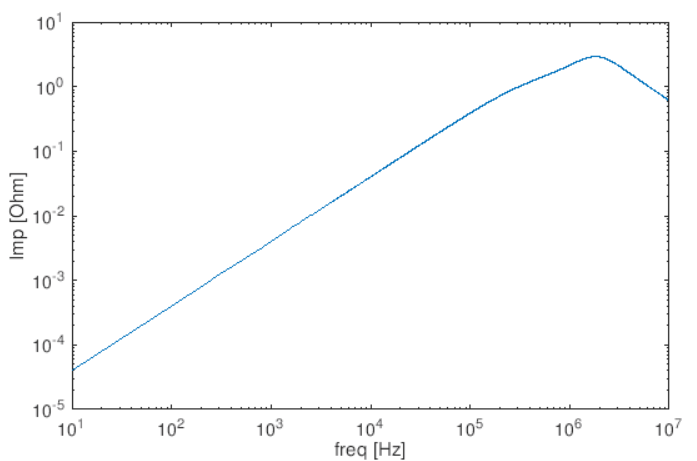
\includegraphics[width=80mm]{fig.png}
  \label{fig1}
  \caption{サンプル図}
\end{figure}

\begin{table}[!htbp]
  \begin{center}
    \label{table1}
	\caption{サンプル}
    \begin{tabular}{|c|c|c|c|}
	\hline
	Pattern & A & B & C \\
	\hline
	Time[ms] & 0.12 & 0.15 & 0.16 \\
	\hline
    \end{tabular}
  \end{center}
\end{table}

\begin{eqnarray}
y = x^2+2 \label{eq1}
\end{eqnarray}


\section{おわりに}
その他,必要に応じて指導教員に確認して論文を作成すること.

\begin{thebibliography}{99}
%\bibitem{ohno}
%大野義夫編,\TeX\ 入門,
%共立出版,東京,1989. 

%\bibitem{Seroul}
%R. Seroul and S. Levy, A Beginner's Book of \TeX, 
%Springer-Verlag, New York, 1989. 

%\bibitem{nodera1}
%野寺隆志,楽々\LaTeX{},
%共立出版,東京,1990. 

\bibitem{Okumura}
奥村晴彦,[改訂版] \LaTeXe\ 美文書作成入門,技術評論社,東京,2000.
\bibitem{Okumura}
(雑誌の場合) 著者名,“標題” ,雑誌名,巻,号,pp.を付けて始め-終りのページ,月(英語)年.
\bibitem{Okumura}
(雑誌例1) 山上一郎,山下二郎,“パラメトリック増幅器”,信学論(B),vol.J62-B,no.1,pp.20-27,Jan. 1979.
\bibitem{Okumura}
(著書,編書の場合) 著者名,書名,編者名,発行所,発行年.
\bibitem{Okumura}
(著書,編書例1) 山田太郎,移動通信,木村次郎(編),pp.21-41,(社)電子情報通信学会,1989.
\bibitem{Okumura}
(国際会議の場合) 著者名,“表題,” 会議名,No.を付けて論文番号,pp.を付けて始め-終りのページ,国名,月(英語)年.
\bibitem{Okumura}
(国際会議例) Y. Yamamoto, S. Machida, and K. Igeta, “Micro-cavity semiconductors with enhanced spontaneous emission,” Proc. 16th European Conf. on Opt. Commun., No. MoF4.6, pp.3-13, Sept. 1990.
\bibitem{Okumura}
(国内大会,研究会論文集例) 川上三郎,川口四郎,“紫外域半導体レーザ”,信学全大,分冊2,No. SB2-1,pp.20-21,Sept. 1995.

\end{thebibliography}


\end{document}
